% ==============================================================================
% PAGE 20: 5) FLOW CONTROL VALVE (Hoffman Clamp Arrangement) (Numbered Page 12)
% ==============================================================================
\subsubsection*{5) FLOW CONTROL VALVE (Hoffman Clamp Arrangement)}

\begin{center}
  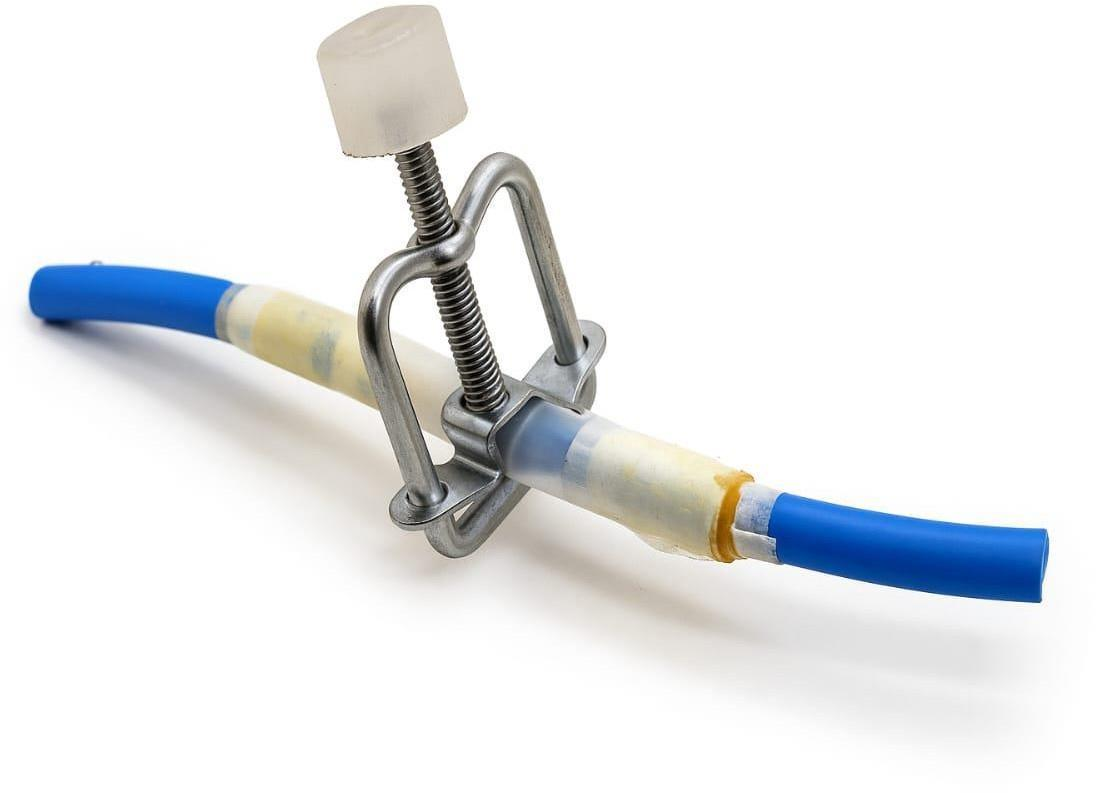
\includegraphics[width=80mm]{figures/fig5_flow_control_valve.jpg}
\end{center}

\noindent
\begin{spacing}{1.2}
{\fontsize{10.2}{14.5}\selectfont
A Hoffman clamp is used in the project as a manual flow control valve for the water passing through the blue supply pipe. It allows precise regulation of the water flow from the storage tank to the copper receiver tube, ensuring that the heating process remains efficient and steady.\\[3mm]
\textbf{Construction:}
\begin{itemize}[leftmargin=8mm, itemsep=1.5mm, label=\textbullet]
  \item The clamp consists of a U-shaped metal frame with a threaded screw and a knob at the top.
  \item The blue flexible pipe passes through the clamp opening.
  \item By rotating the knob clockwise, the screw presses against the pipe, restricting or stopping the water flow.
  \item Turning it anti-clockwise loosens the pressure, allowing smooth water passage.
\end{itemize}
\vspace{2mm}
\textbf{Function in the Project:}
\begin{enumerate}[leftmargin=8mm, itemsep=2mm]
  \item Controls the rate of water flow to maintain proper heat absorption in the copper tube.
  \item Prevents wastage of hot water and maintains uniform temperature rise.
  \item Acts as a simple and low-cost valve system, eliminating the need for expensive plumbing fittings.
  \item Makes the experimental setup easy to adjust during testing. This component ensures better temperature control and improves the overall performance and efficiency of the solar water heater.
\end{enumerate}
}
\end{spacing}
\clearpage
